%%% Please replace what is within each curly bracket with the correct information below. %%%
%%% The first field is already filled in for you.  %%%
\def\ClassName {CS188} % Your course 
\def\NameLast {Jois}  % Your last name
\def\NameFirst {Manohar}  % Your first name
\def\SID{23808180}  % Your SID
\def\Email{m.k.jois@berkeley.edu} % Your pandagrader email
\def\Collaborators{} % Any collaborators


%%%%% FILL IN YOUR ANSWERS TO EACH QUESTION BY REPLACE WHAT IS IN THE CURLY BRACKETS.
\def\AnswerOneAi{\textbf{Put your answer to 1ai here:} 
%%% Begin 1a answer
The variables are $q_1, \ldots, q_6$ for the six questions, which can each take on a value in $\{1,2,3\}$ for John, Kevin and Anna, respectively.
\begin{align*}
q_1 &\in \{1,2,3\} \\
q_2 &\in \{1,2\} \\
q_3 &\in \{1,2,3\} \\
q_4 &\in \{1\} \\
q_5 &\in \{1,3\} \\
q_6 &\in \{1\}
\end{align*}
%%% End 1a answer
}
\def\AnswerOneAii{\textbf{Put your answer to 1aii here:}
%%% Begin 1b answer
\\
\begin{tabular}{cc}
$q_4 \neq 2$ & $q_4 = q_6$ \\
$q_5 \neq 2$ & $q_1 \neq q_2$ \\
$q_6 \neq 2$ & $q_2 \neq q_3$ \\
$q_2 \neq 3$ & $q_3 \neq q_4$ \\
$q_4 \neq 3$ & $q_4 \neq q_5$ \\
$q_6 \neq 3$ & $q_5 \neq q_6$
\end{tabular}
%%% End 1b answer 
}
\def\AnswerOneB{\textbf{Put your answer(s) to 1b here:}\\
%%% Begin 1c answer
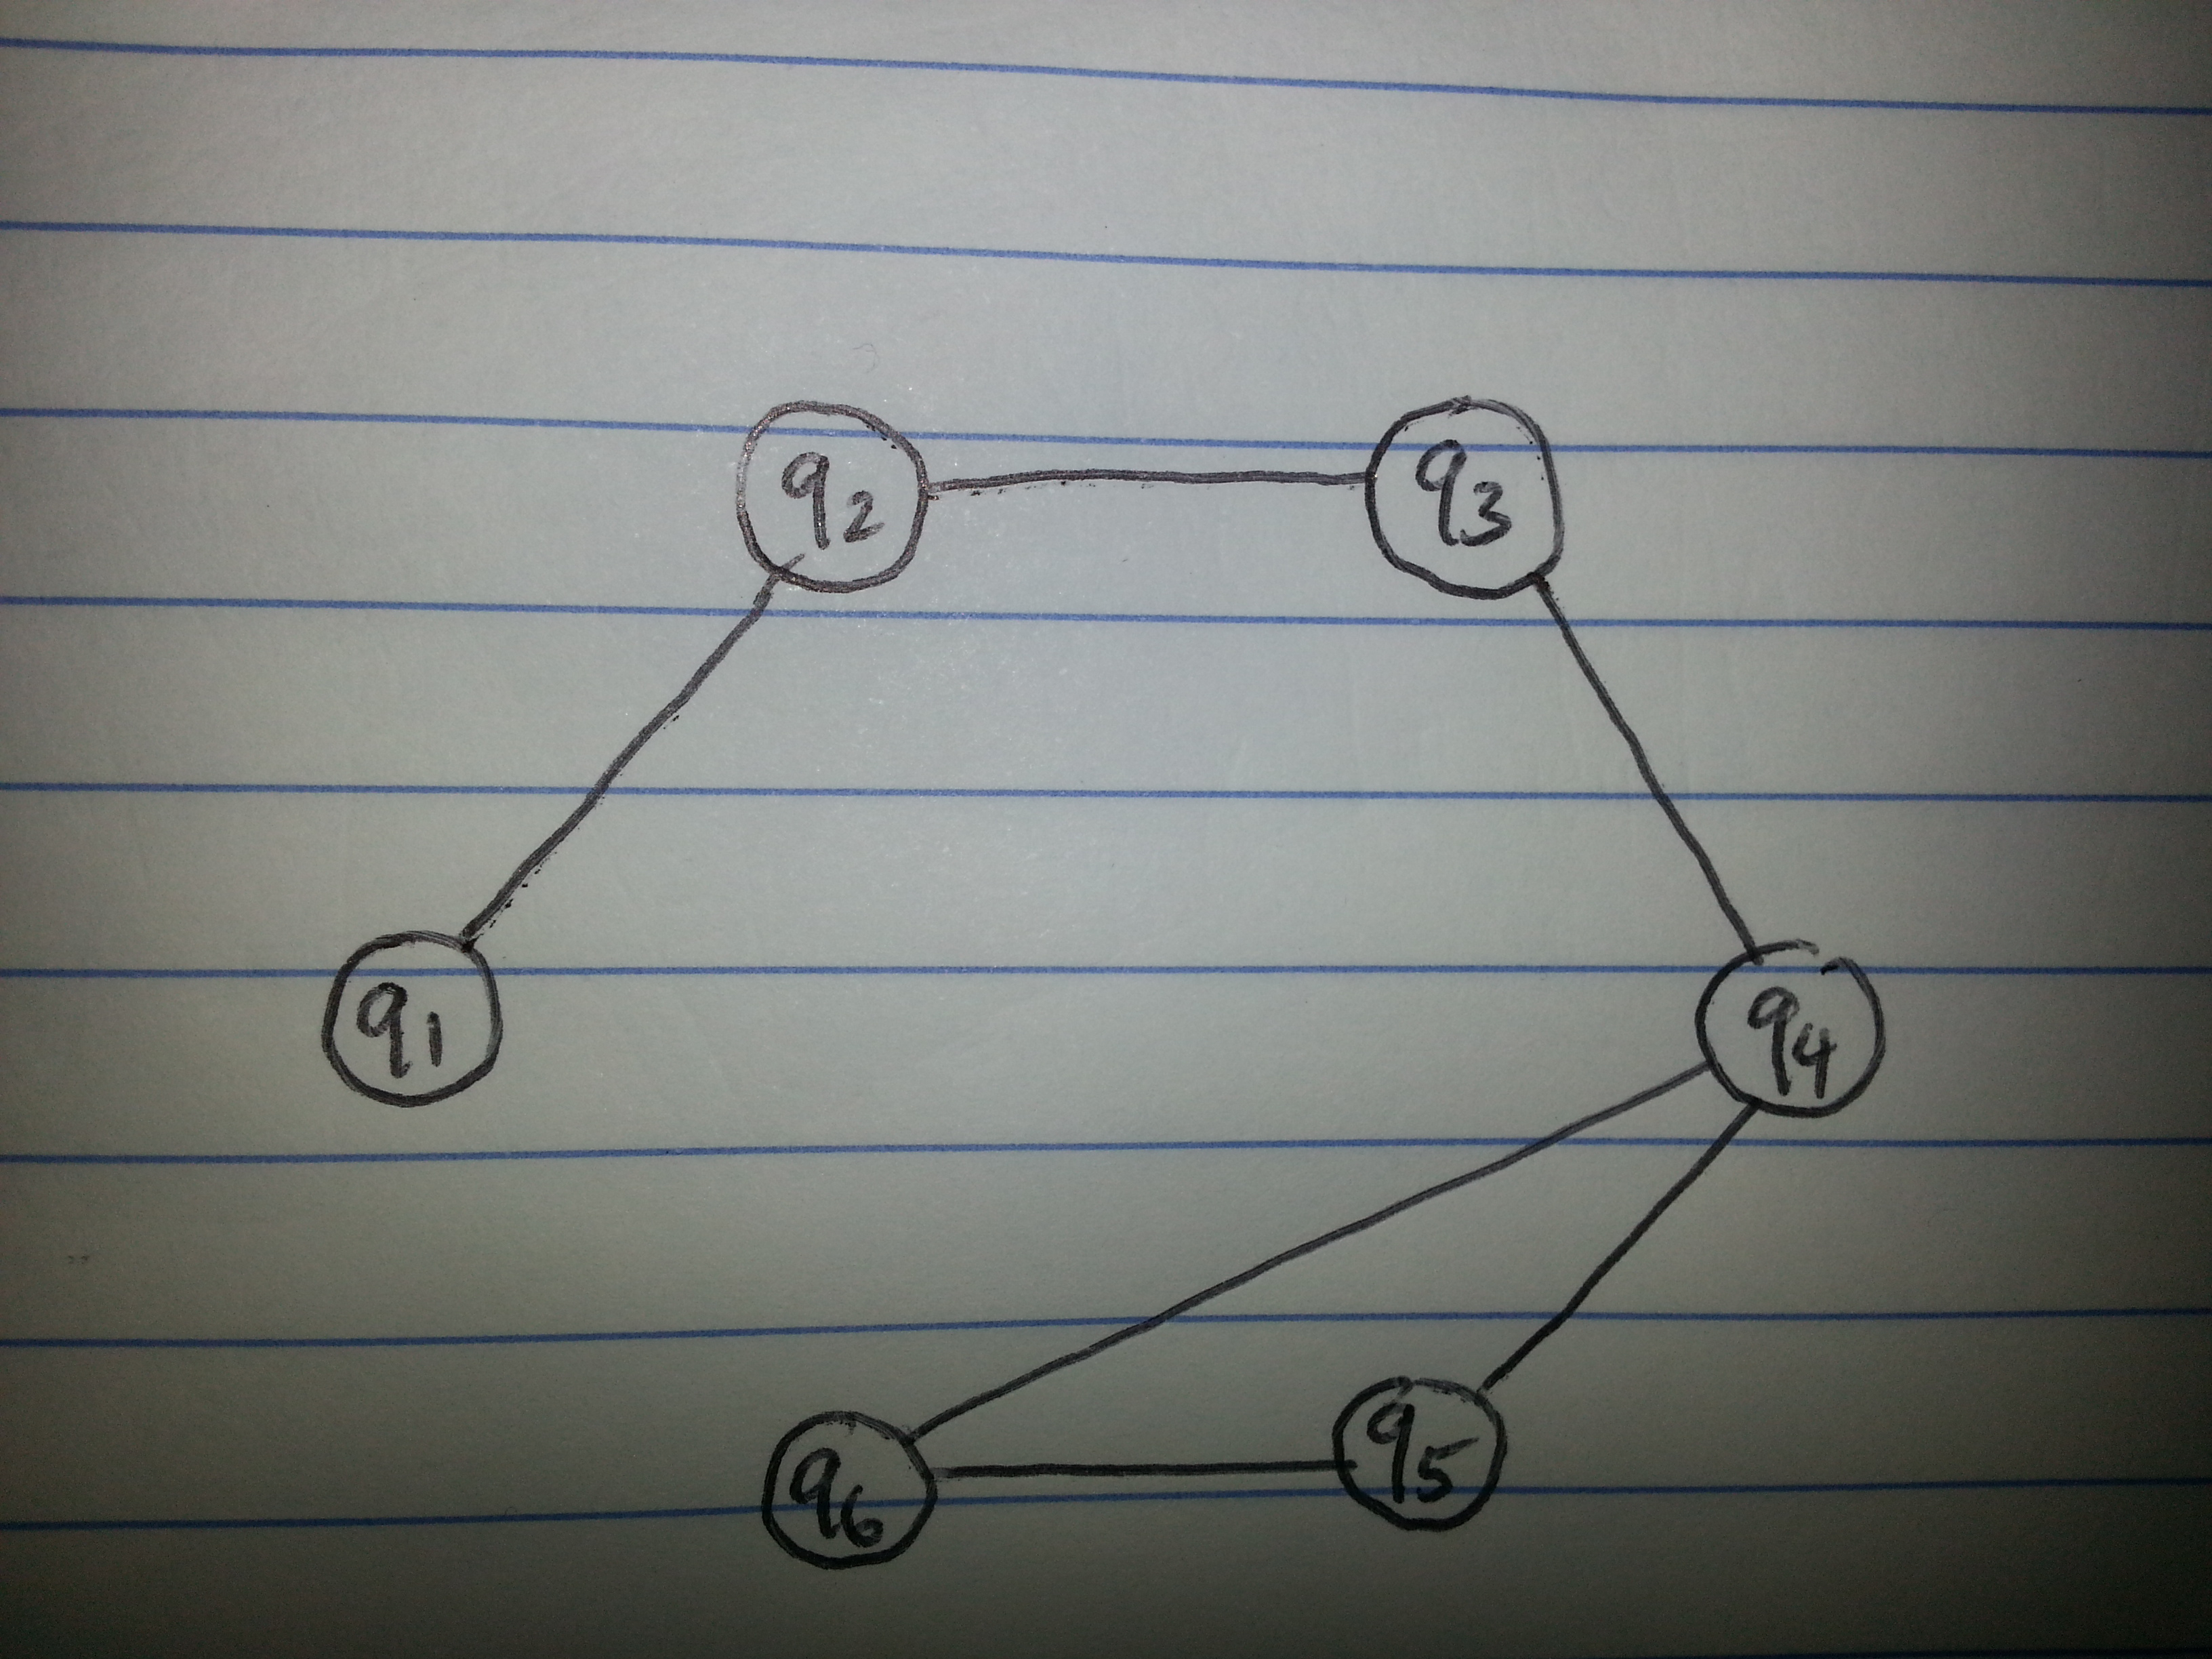
\includegraphics[scale=0.07]{figures/q1b}
%%% End 1c answer 
}

\def\AnswerTwoAi{
%%% Use \cross{1} to cross out a number
\begin{tabular}{ccccccc}
P & \cross{1} & \cross{2} & \cross{3} & 4 & 5 & 6\\
B & \cross{1} & 2 & \cross{3} & 4 & \cross{5} & 6\\
C & 1 & 2 & 3 & 4 & 5 & 6\\
K & \cross{1} & 2 & 3 & 4 & 5 & \cross{6}\\
I & 1 & 2 & 3 & 4 & 5 & 6\\
M & \cross{1} & \cross{2} & \cross{3} & \cross{4} & 5 & 6\\
\end{tabular}
}

\def\AnswerTwoAii{
%%% Replace '\Circle' with '\CIRCLE' to color in the bubble
\Circle \hspace{0.2cm} P \hfill
\Circle \hspace{0.2cm} B \hfill
\Circle \hspace{0.2cm} C \hfill
\Circle \hspace{0.2cm} K \hfill
\Circle \hspace{0.2cm} I \hfill
\CIRCLE \hspace{0.2cm} M \hfill\\
}

\def\AnswerTwoAiii{
%%% Use \cross{1} to cross out a number
\begin{tabular}{ccccccc}
P &   &   &   &  &   &  6\\
B & \cross{1} & \cross{2} & \cross{3} & 4 & \cross{5} & \cross{6}\\
C & 1 & 2 & 3 & 4 & 5 & \cross{6}\\
K & \cross{1} & 2 & 3 & 4 & 5 & \cross{6}\\
I & 1 & 2 & 3 & 4 & 5 & \cross{6}\\
M & \cross{1} & \cross{2} & \cross{3} & \cross{4} & 5 & \cross{6}\\
\end{tabular}
}

\def\AnswerTwoAivPartOne{
\begin{tabular}{|c|c|}
\hline
Variable & \# violated\\
\hline
P & 0%Insert number here% 
\\\hline
B & 0%Insert number here% 
\\\hline
C & 1%Insert number here% 
\\\hline
K & 0%Insert number here% 
\\\hline
I & 2%Insert number here% 
\\\hline
M & 0%Insert number here% 
\\\hline
\end{tabular}
}

\def\AnswerTwoAivPartTwo{
%%% Answer by placing 'x' in correct grids
\begin{tabular}{|c|c|c|c|c|c|c|}
\hline & 1 & 2 & 3 & 4 & 5 & 6 
\\\hline
P & & & & & &
\\\hline
B & & & & & &
\\\hline
C & & x & & & &
\\\hline
K & & & & & &
\\\hline
I & & x & x & x & x &
\\\hline
M & & & & & &
\\\hline
\end{tabular}
}

%%% Replace '\Circle' with '\CIRCLE' to color in the bubble
\def\AnswerThreeA{
\CIRCLE \hspace{0.2cm} Neither MRV nor LCV can have an effect.\\\\ &
\Circle \hspace{0.2cm} Only MRV can have an effect.\\\\ &
\Circle \hspace{0.2cm} Only LCV can have an effect .\\\\ &
\Circle \hspace{0.2cm} Both MRV and LCV can have an effect.\\\\
}
\def\AnswerThreeB{
\Circle \hspace{0.2cm} Neither MRV nor LCV can have an effect.\\\\ &
\CIRCLE \hspace{0.2cm} Only MRV can have an effect.\\\\ &
\Circle \hspace{0.2cm} Only LCV can have an effect .\\\\ &
\Circle \hspace{0.2cm} Both MRV and LCV can have an effect.\\\\
}
\def\AnswerThreeC{
\Circle \hspace{0.2cm} Neither MRV nor LCV can have an effect.\\\\ &
\CIRCLE \hspace{0.2cm} Only MRV can have an effect.\\\\ &
\Circle \hspace{0.2cm} Only LCV can have an effect .\\\\ &
\Circle \hspace{0.2cm} Both MRV and LCV can have an effect.\\\\
}
\def\AnswerThreeD{
\Circle \hspace{0.2cm} Neither MRV nor LCV can have an effect.\\\\ &
\CIRCLE \hspace{0.2cm} Only MRV can have an effect.\\\\ &
\Circle \hspace{0.2cm} Only LCV can have an effect .\\\\ &
\Circle \hspace{0.2cm} Both MRV and LCV can have an effect.\\\\
}
\def\AnswerThreeE{
\Circle \hspace{0.2cm} Neither MRV nor LCV can have an effect.\\\\ &
\CIRCLE \hspace{0.2cm} Only MRV can have an effect.\\\\ &
\Circle \hspace{0.2cm} Only LCV can have an effect .\\\\ &
\Circle \hspace{0.2cm} Both MRV and LCV can have an effect.\\\\
}

%%%%%%%%%%%%%%%%%%%%%% DO NOT CHANGE ANYTHING BELOW THIS LINE %%%%%%%%%%%%%%%%%%%%%%%%%
\documentclass[written]{cs188}

\usepackage{verbatim}
\usepackage{fancyhdr}
\usepackage{booktabs}
\usepackage{setspace}
\usepackage{amsmath,mathrsfs}
\usepackage{multicol}
\usepackage{amssymb}
\usepackage{algpseudocode}
\usepackage{graphicx}
\usepackage{caption}
\usepackage{subcaption}
\usepackage{array}
\usepackage{xcolor}
\usepackage{float}
\usepackage{enumitem}
\usepackage{mathcomp}
\usepackage{tabularx}
\usepackage{wasysym}
\usepackage{pbox}
\usepackage{tikz}
\usetikzlibrary{matrix}
\usepackage[normalem]{ulem}
\usepackage{multirow}

% Bubbles for multiple choice questions
\newcommand{\mcqbubble}{\bigcirc}
\newcommand{\mcqbubblefill}{\Large\newmoon}

% shorthand
\newcommand{\mcqb}{$\bigcirc$\ \ }
\newcommand{\mcqs}{\solution{\mcqb}{$\Large\newmoon$\ \ }}

% pruning
\newcommand{\prune}{\includegraphics[width=0.2in]{figures/red_x}}
\title{Written HW4}

\begin{document}

\newpage
\begin{problem}[]{Occupy Cal}

You are at Occupy Cal, and the leaders of the protest are deciding whether or not to march on California Hall. The decision is made centrally and communicated to the occupiers via the ``human microphone''; that is, those who hear the information repeat it so that it propagates outward from the center. This scenario is modeled by the following Bayes net:

\vspace{2mm}
\begin{figure}[htp]
\centering
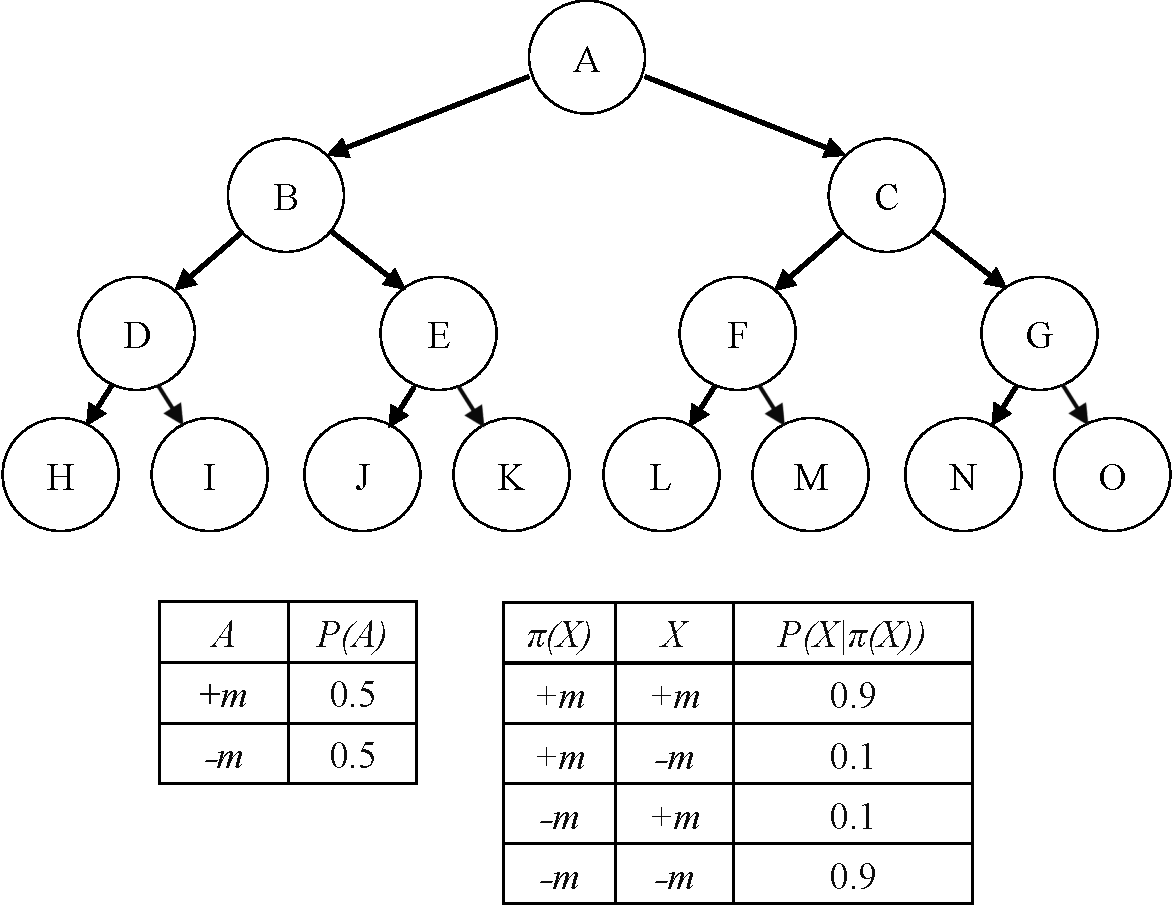
\includegraphics[width=105mm]{figures/tree-labeled-tables-crop.pdf}
\end{figure}
\vspace{2mm}

Each random variable represents whether a given group of protestors hears instructions to march ($+m$) or not ($-m$). The decision is made at $A$, and both outcomes are equally likely. The protestors at each node relay what they hear to their two child nodes, but due to the noise, there is some chance that the information will be misheard. Each node except $A$ takes the same value as its parent with probability 0.9, and the opposite value with probability 0.1, as in the conditional probability tables shown.

\begin{question}[4] Compute the probability that node $A$ sent the order to march ($A = +m$) given that both $B$ and $C$ receive the order to march ($B=+m$, $C=+m$). \\
\fbox{\begin{minipage}[t][4cm][t]{17cm}
\OneA
\end{minipage}}
\end{question}

\begin{question}[4] Compute the probability that $D$ receives the order $+m$ given that $A$ sent the order $+m$. \\
\fbox{\begin{minipage}[t][4cm][t]{17cm}
\OneB
\end{minipage}}
\end{question}

You are at node $D$, and you know what orders have been heard at node $D$. Given your orders, you may either decide to march (\emph{march}) or stay put (\emph{stay}). (Note that these actions are distinct from the orders $+m$ or $-m$ that you hear and pass on. The variables in the Bayes net and their conditional distributions still behave exactly as above.) If you decide to take the action corresponding to the decision that was actually made at $A$ (not necessarily corresponding to your orders!), you receive a reward of $+1$, but if you take the opposite action, you receive a reward of $-1$. \\

\begin{question}[4] Given that you have received the order $+m$, what is the expected utility of your optimal action? (Hint: your answer to part (b) may come in handy.) \\
\fbox{\begin{minipage}[t][5cm][t]{17cm}
\OneC
\end{minipage}}
\end{question}

Now suppose that you can have your friends text you what orders they have received. (Hint: for the following two parts, you should not need to do much computation due to symmetry properties and intuition.)

\begin{question}[4] Compute the VPI of $A$ given that $D = +m$. \\
\fbox{\begin{minipage}[t][5cm][t]{17cm}
\OneD
\end{minipage}}
\end{question}

\begin{question}[4] Compute the VPI of $A$ given that $D = +m$ and $B = -m$. \\
\fbox{\begin{minipage}[t][5cm][t]{17cm}
\OneE
\end{minipage}}
\end{question}

\end{problem}
\newpage
\q{30}{Neural Networks}

In this problem, you are given a simple network that uses the simple linear function $g(x) = mx + b$ (where $m$ and $b$ values are fixed) as the activation function (rather than, for example,  a sigmoid function). You will need to write the $L_2$ norm (squared) loss function, the partial derivative of the loss function, and the gradient descent update rule for certain weights.

\textbf{Single Neuron Example}

We have given you the answers for the loss function, partial derivative, and weight update rule for the following single neuron example. This example should help you understand how to structure your answers to the questions about the slightly more complex network on the following page.

\begin{figure}[h]
\centering
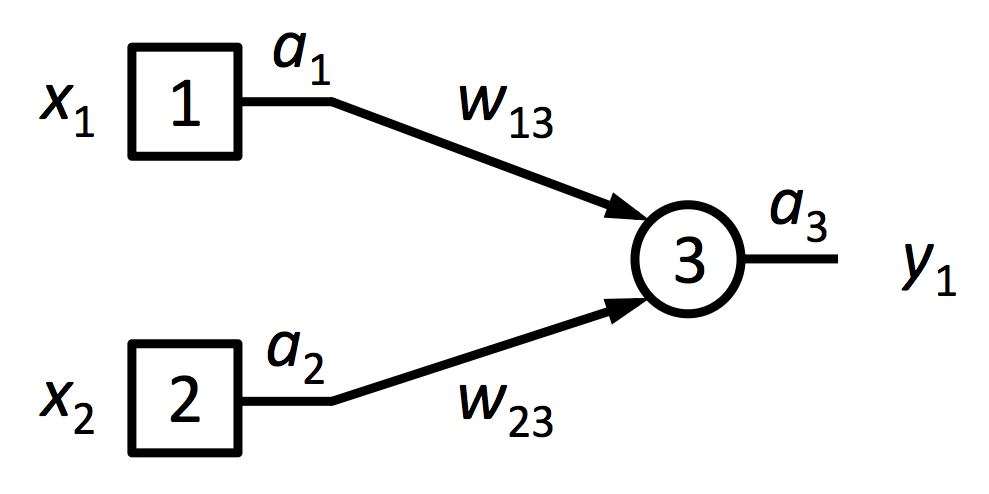
\includegraphics[width=0.25\linewidth]{figs/NN_1.png}
\end{figure}
\begin{flalign*}
a_1 &= x_1 &\\
a_2 &= x_2 &\\
a_3 &= m(w_{13}a_1+w_{23}a_2) + b &
\end{flalign*}
\textbf{Loss function}
\begin{flalign*}
Loss(\boldsymbol{w}) &= ||\boldsymbol{y}-\boldsymbol{h_w}(\boldsymbol{x})||_2^2 &\\
&= (y_1 - a_3)^2 &\\
&= (y_1 - m(w_{13}a_1+w_{23}a_2) - b)^2 &\\
&= (y_1 - m(w_{13}x_1+w_{23}x_2) - b)^2 &
\end{flalign*}
\textbf{Loss partial derivative}
\begin{flalign*}
\frac{\partial }{\partial w_{13}}Loss(\boldsymbol{w}) &= -2(y_1 - a_3) \frac{\partial a_3}{\partial w_{13}} &\\
&= -2(y_1 - a_3)ma_1 &\\
&= -2(y_1 - m(w_{13}x_1+w_{23}x_2) - b)mx_1 &
\end{flalign*}
\textbf{Weight update rule}
\begin{flalign*}
w_{13} &\leftarrow w_{13} - \alpha \frac{\partial }{\partial w_{13}} Loss(\boldsymbol{w})&\\
&= w_{13} + \alpha 2(y_1 - m(w_{13}x_1+w_{23}x_2) - b)mx_1 &
\end{flalign*}

(Question continued on next page)

\newpage
\textbf{Simple Neural Network with Linear Activation Function}

Given the following neural network (again, using the simple linear activation function $g(x) = mx + b$):

\begin{figure}[h]
\centering
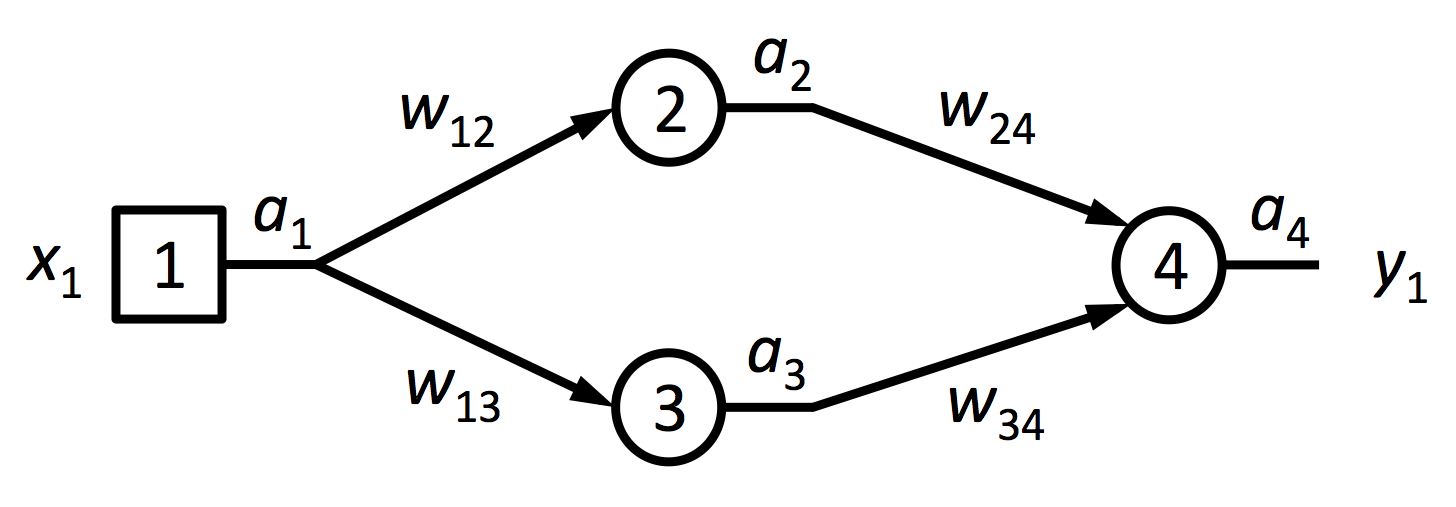
\includegraphics[width=0.4\linewidth]{figs/NN_2.png}
\end{figure}

\begin{question}{[5 pts]}
Write the loss function, $Loss(\boldsymbol{w})$, in terms of $x_1$, $y_1$, $w_{12}$, $w_{13}$, $w_{24}$, $w_{34}$, $m$, and $b$.

\begin{minipage}{\textwidth}
    \solution{} {\begin{align*}
    Loss(\boldsymbol{w}) &= (y_1-a_4)^2\\
    &= (y_1-m(w_{24}a_2+w_{34}a_3)-b)^2\\
    &= (y_1-m(w_{24}(mw_{12}a_1+b)+w_{34}(mw_{13}a_1+b))-b)^2\\
    &= (y_1-m^2w_{12}w_{24}x_1-mw_{24}b-m^2w_{13}w_{34}x_1-mw_{34}b-b)^2
    \end{align*}
    }
\end{minipage}

\end{question}

\begin{question}{[5 pts]}
Write the derivative of the loss function with respect to $w_{24}$, $\frac{\partial}{\partial w_{24}} Loss(\boldsymbol{w})$, in terms of $x_1$, $y_1$, $w_{12}$, $w_{13}$, $w_{24}$, $w_{34}$, $m$, and $b$.

\begin{minipage}{\textwidth}
    \solution{} {\begin{align*}
    \frac{\partial}{\partial w_{24}}Loss(\boldsymbol{w}) &= -2(y_1-a_4)\frac{\partial a_4}{\partial w_{24}}\\
    &= -2ma_2(y_1-a_4)\\
    &= -2m(mw_{12}x_1+b)(y_1-m^2w_{12}w_{24}x_1-mw_{24}b-m^2w_{13}w_{34}x_1-mw_{34}b-b)
    \end{align*}
    }
\end{minipage}

\end{question}

\begin{question}{[2 pts]}
Write the gradient descent update rule for $w_{24}$ with step size $\alpha$ in terms of $\alpha$ $x_1$, $y_1$, $w_{12}$, $w_{13}$, $w_{24}$, $w_{34}$, $m$, and $b$.

\begin{minipage}{\textwidth}
    \solution{} {\begin{align*}
    w_{24} &\leftarrow w_{24}-\alpha\frac{\partial}{\partial w_{24}} Loss(\boldsymbol{w})\\
    &= w_{24}+2\alpha m(mw_{12}x_1+b)(y_1-m^2w_{12}w_{24}x_1-mw_{24}b-m^2w_{13}w_{34}x_1-mw_{34}b-b)
    \end{align*}
    }
\end{minipage}

\end{question}

\begin{question}{[5 pts]}
Write the derivative of the loss function with respect to $w_{12}$, $\frac{\partial}{\partial w_{12}} Loss(\boldsymbol{w})$, in terms of $x_1$, $y_1$, $w_{12}$, $w_{13}$, $w_{24}$, $w_{34}$, $m$, and $b$.

\begin{minipage}{\textwidth}
    \solution{} {\begin{align*}
    \frac{\partial}{\partial w_{12}}Loss(\boldsymbol{w}) &= -2(y_1-a_4)\frac{\partial a_4}{\partial w_{12}}\\
    &= -2(y_1-a_4)(mw_{24}\frac{\partial a_2}{\partial w_{12}}+mw_{34}\frac{\partial a_3}{\partial w_{12}})\\
    &= -2(y_1-a_4)(mx_1+0)\\
    &= -2mx_1(y_1-m^2w_{12}w_{24}x_1-mw_{24}b-m^2w_{13}w_{34}x_1-mw_{34}b-b)
    \end{align*}
    }
\end{minipage}

\end{question}

\begin{question}{[2 pts]}
Write the gradient descent update rule for $w_{12}$ with step size $\alpha$ in terms of $\alpha$ $x_1$, $y_1$, $w_{12}$, $w_{13}$, $w_{24}$, $w_{34}$, $m$, and $b$.

\begin{minipage}{\textwidth}
    \solution{} {\begin{align*}
    w_{12} &\leftarrow w_{12}-\alpha\frac{\partial}{\partial w_{12}} Loss(\boldsymbol{w})\\
    &= w_{12}+2\alpha mx_1(y_1-m^2w_{12}w_{24}x_1-mw_{24}b-m^2w_{13}w_{34}x_1-mw_{34}b-b)
    \end{align*}
    }
\end{minipage}
\end{question}

\newpage

\begin{question}{[3 pts]}
Because this network has a linear activation function, there is an equivalent network that has no hidden layers. 1) Draw a new (very simple) network that has no hidden layers but computes exactly the same function. 2) Write the new weight explicitly in terms of the $w_{12}$, $w_{13}$, $w_{24}$, $w_{34}$, $m$, and $b$. 3) You will need to adjust the linear activation function, $g_2(x) = m_2x + b_2$. Write the new $m_2$ and $b_2$ values in terms of $w_{12}$, $w_{13}$, $w_{24}$, $w_{34}$, $m$, and $b$.

\begin{minipage}{\textwidth}
    \solution{} {\begin{verbatim}
    x1 (1) a1 -----------> (2) a2', y1
                   w'
    \end{verbatim}
    \begin{align*}
    a2' &= a4\\
    &= m^2w_{12}w_{24}x_1+mw_{24}b+m^2w_{13}w_{34}x_1+mw_{34}b+b\\
    &= m^2(w_{12}w_{24}+w_{13}w_{34})x_1 + (mw_{24}b+mw_{34}b+b)\\
    w' &= w_{12}w_{24}+w_{13}w_{34}\\
    m_2 &= m^2\\
    b_2 &= mw_{24}b+mw_{34}b+b
    \end{align*}
    }
\end{minipage}
\end{question}

\textbf{General Neural Network with Linear Activation Function}

\vspace{3mm}
Consider a new neural network with $n$ input nodes, $n$ output nodes, one hidden layer with $h$ nodes, and the linear activation function $g(x) = mx + b$ at each hidden and output node. The nodes between each layer are fully connected with weights $w_{ij}$ from the $i$-th input node to the $j$-th hidden node and weights $w_{jk}$ from the $j$-th hidden node to the $k$-th output node.

\vspace{3mm}
\begin{question}{[5 pts]}
Because this general network has a linear activation function, there is an equivalent network that has no hidden layers that computes exactly the same function. 1) Write an equation for the weight $w_{ik}$ from the $i$-th input node to the $k$-th output node explicitly in terms of the previous network weights ($w_{ij}$, $w_{jk}$), $m$, and $b$. 2) You will need to adjust the linear activation function, $g_2(x) = m_2x + b_2$. Write the new $m_2$ and $b_2$ values in terms of the previous network weights ($w_{ij}$, $w_{jk}$), $m$, and $b$.

\begin{minipage}{\textwidth}
    \solution{} {\begin{align*}
    y_k &= m\sum_{j=1}^h(w_{jk}(m\sum_{i=1}^n(w_{ij}x_i)+b))+b\\
    &= m^2\left(\sum_{j=1}^h\sum_{i=1}^n w_{ij}w_{jk}x_i\right) + \left(\sum_{j=1}^h\sum_{i=1}^n mw_{jk}b\right) + b\\
    w_{ik} &= \sum_{j=1}^h w_{ij}w_{jk}\\
    m_2 &= m^2\\
    b_{2,k} &= b\left(1+mn\sum_{j=1}^h w_{jk}\right)
    \end{align*}
    }
\end{minipage}
\end{question}

\begin{question}{[3 pts]}
What effect does removing the hidden layer from this general network have on the number of weights? Specifically, in terms of $n$ and $h$, how many weights are there before and after removing the hidden layer? Discuss in particular the case when $h << n$.

\begin{minipage}{\textwidth}
    \solution{} {
    \paragraph{} Before removing the hidden layer there are $hn$ weights on each side of it for a total of $2hn$ weights. After removing it, there are $n^2$ weights, one for each pair of input/output. When $h<<n$ this essentially increases the number of weights by a factor of $\frac n2$.
    }
\end{minipage}

\end{question}





\newpage
\begin{problem}{All Satisfying Assignments}
Consider a modified CSP in which we wish to find every possible satisfying assignment, rather than just one such assignment as in normal CSPs. In order to solve this new problem, consider a new algorithm which is the same as the normal backtracking search algorithm, except that when it sees a solution, instead of returning it, the solution gets added to a list, and the algorithm backtracks. Once there are no variables remaining to backtrack on, the algorithm returns the list of solutions it has found.\\\\
For each graph below, select whether or not using the MRV and/or LCV heuristics could affect the number of nodes expanded in the search tree in this new situation.

\begin{question}[8]{}\\
\begin{tabular}{cl}
&\\
\multirow{1}{*}{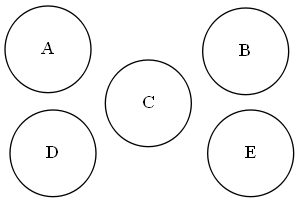
\includegraphics[scale=0.5]{figures/disconnected.png} \hspace{1.4in}} &
\AnswerThreeA
\end{tabular}\\
\end{question}

\vspace{-.2in}
\begin{question}[8]{}\\
\begin{tabular}{cl}
\multirow{1}{*}{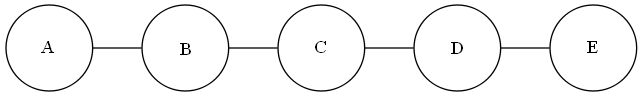
\includegraphics[width=3in]{figures/chain.png}} &
\AnswerThreeB
\end{tabular}\\
\end{question}

\vspace{-.2in}
\begin{question}[8]{}\\
\begin{tabular}{cl}
\multirow{1}{*}{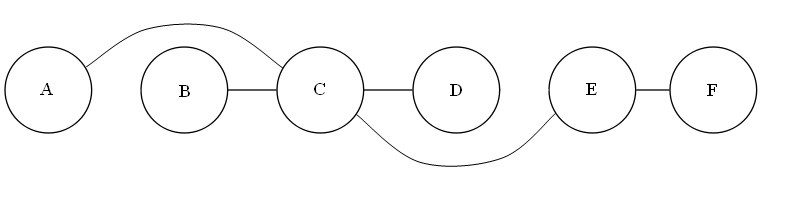
\includegraphics[width=3in]{figures/tree.png}} &
\AnswerThreeC
\end{tabular}
\end{question}

\vspace{-.2in}
\begin{question}[8]{}\\
\begin{tabular}{cl}
\multirow{1}{*}{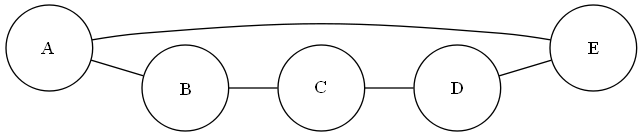
\includegraphics[width=3in]{figures/circle.png}} &
\AnswerThreeD
\end{tabular}
\end{question}

\vspace{-.2in}
\begin{question}[8]{}\\
\begin{tabular}{cl}
\multirow{1}{*}{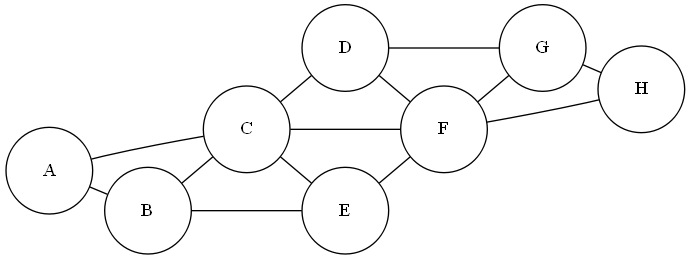
\includegraphics[width=3in]{figures/csp_graph.png}} &
\AnswerThreeE
\end{tabular}
\end{question}

\end{problem}

\end{document}